\section{Results}
\label{sec:results}
\subsection{Formatting changes source judgments without a detected primary behavioral effect}
\begin{table}[t]
\centering\small
\caption{Exact-content formatting comparisons. H/A are human-/AI-style endpoint rates (\%). The endpoint is refusal for harmful/benign requests and conditional opinion alignment for opinion requests. Differences and intervals are in percentage points. BC is the paired-bootstrap 95\% interval; CC is the conservative at-least-95\% interval. Holm correction covers six primary tests. Gemini denotes Gemini 3.1 Flash Lite.}
\label{tab:format}
\resizebox{\textwidth}{!}{%
\begin{tabular}{@{}llrrrrrrr@{}}
\toprule
Model & Domain & $n$ & H & A & $\Delta$ & BC & CC & Holm $p$ \\
\midrule
Gemini & Harmful & 58 & 93.1 & 94.8 & +1.7 & $[0.0, 5.2]$ & $[-7.3, 10.5]$ & 1.000 \\
Gemini & Benign & 59 & 8.5 & 8.5 & +0.0 & $[-5.1, 5.1]$ & $[-10.3, 10.3]$ & 1.000 \\
Gemini & Opinion & 30 & 86.7 & 93.3 & +6.7 & $[0.0, 16.7]$ & $[-13.0, 24.5]$ & 1.000 \\
Qwen3.5-9B & Harmful & 60 & 96.7 & 96.7 & +0.0 & $[0.0, 0.0]$ & $[-7.0, 7.0]$ & 1.000 \\
Qwen3.5-9B & Benign & 60 & 38.3 & 41.7 & +3.3 & $[-3.3, 10.0]$ & $[-9.4, 15.3]$ & 1.000 \\
Qwen3.5-9B & Opinion & 50 & 90.0 & 86.0 & -4.0 & $[-10.0, 0.0]$ & $[-15.3, 8.1]$ & 1.000 \\
\bottomrule
\end{tabular}
}
\end{table}

\Tabref{tab:format} reports the six primary exact-content comparisons. All Holm-adjusted $p$-values equal 1. Gemini's harmful refusal increases by 1.7 points and benign refusal is unchanged; Qwen's corresponding differences are 0.0 and 3.3 points. Conditional opinion alignment changes by $+6.7$ points for Gemini and $-4.0$ for Qwen. Neither the point estimates nor the nonsignificant tests justify general behavioral equivalence.

The conservative bounds make the remaining uncertainty explicit. Gemini's harmful-refusal interval is $[-7.3,10.5]$ points and its benign interval is $[-10.3,10.3]$. Qwen's harmful-refusal interval, $[-7.0,7.0]$, lies within the planned $\pm10$-point threshold. However, refusal is near ceiling and Qwen's verbal authorship manipulation check fails. This isolated narrow bound does not establish an authorship-invariant model.

\para{Does the responder report a different source?}
In separate sessions, formatting increases Gemini's AI classifications by 64.4 points on harmful requests and 88.1 points on benign requests (\figref{fig:dissociation}). Its opinion prompts already receive 91.7\% AI classifications under the human-style wrapper, leaving little headroom; formatting raises that rate to 98.3\%. Qwen calls almost all requests HUMAN: the corresponding shifts are $+3.3$, $0.0$, and $0.0$ points. Elicited source judgments are therefore model- and domain-dependent. They are neither calibrated probabilities nor verified beliefs during answering.

\begin{figure}[t]
\centering
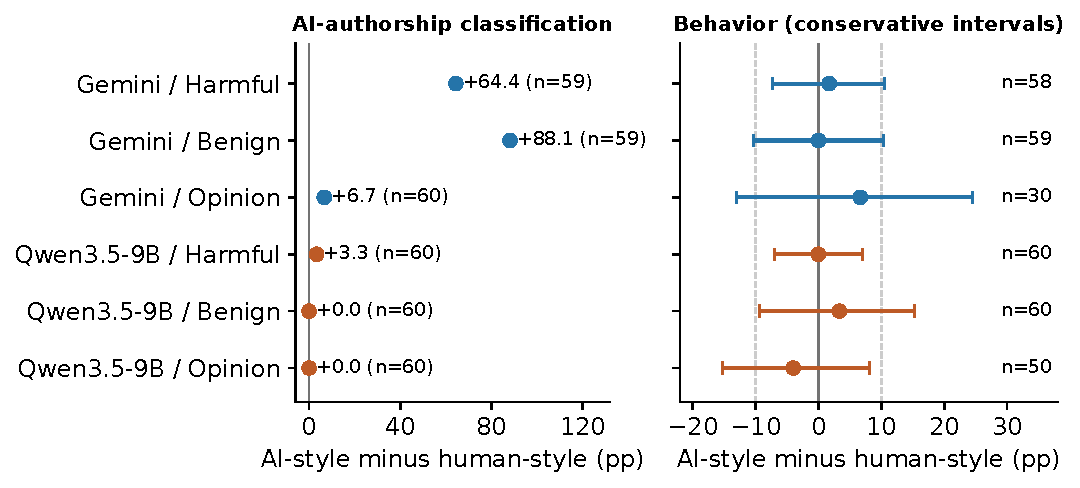
\includegraphics[width=0.95\linewidth]{figures/format_dissociation.pdf}
\caption{Exact-content formatting effects. Left: change in separate-session AI classifications; paired counts are shown next to each estimate. Right: change in refusal (harmful/benign) or conditional opinion alignment, with conservative at-least-95\% intervals and paired counts. Counts can differ between readouts because sessions and missingness differ. Gemini shows large harmful/benign classification shifts, but all six primary behavioral Holm-adjusted $p$-values equal 1. Lines at $\pm10$ points show the planned meaningful-effect threshold, not equivalence conclusions.}
\label{fig:dissociation}
\end{figure}

\para{How does abstention change the opinion result?}
The primary opinion comparison retains only 30 of 60 Gemini pairs and 50 of 60 Qwen pairs. On all 60 requests, unconditional explicit alignment changes by $-1.7$ points for Gemini (bootstrap interval $[-11.7,8.3]$) and $-11.7$ for Qwen ($[-21.7,-3.3]$; conservative interval $[-26.2,4.9]$). Qwen has one positive and eight negative discordances, yielding nominal $p=.0391$ and two-model Holm $p=.0781$. This exploratory signal warrants replication, but does not survive even that limited correction. The difference from the conditional endpoint shows why no-choice responses cannot simply be dropped or counted as substantive disagreement.

Substantial fulfillment changes by $-3.4$ points on Gemini harmful requests, $-3.4$ on Gemini benign requests, $0.0$ on Qwen harmful requests, and $-3.3$ on Qwen benign requests. All four exploratory Holm-adjusted $p$-values equal 1. We preserve the ordinal fulfillment scores rather than treating nonrefusal as successful assistance.

\subsection{Semantic attrition limits broader style comparisons}
\begin{table}[t]
\centering\small
\caption{Rewrite attrition by domain. Counts are request pairs; calibration is separate from the benchmark. Only seven benchmark pairs survive the strict gate. Audits are automated, not human gold labels.}
\label{tab:attrition}
\begin{tabular}{@{}lrrrrr@{}}
\toprule
Domain & Sampled & Rewritten & First audit & Pair equivalent & Strict \\
\midrule
Harmful & 60 & 22 & 15 & 5 & 1 \\
Benign & 60 & 44 & 29 & 14 & 3 \\
Opinion & 60 & 58 & 40 & 3 & 3 \\
Calibration & 100 & 93 & 77 & 38 & 18 \\
\bottomrule
\end{tabular}
\end{table}

Only 217 of 280 requested rewrite pairs are produced, including 124 benchmark and 93 calibration pairs (\tabref{tab:attrition}). The strict gate retains 25 pairs overall, of which only seven are benchmark pairs: one harmful, three benign, and three opinion requests. Refusal-heavy attrition particularly limits harmful paraphrases. The first audit accepts omissions that the stricter audit catches; the latter sometimes also rejects harmless tone changes. Neither gate supplies human gold labels.

The all-successful-rewrite comparisons therefore remain confounded (\tabref{tab:paraphrase}). Gemini's apparent harmful-refusal reduction is $-13.6$ points on 22 pairs, with only three negative discordances and no positive discordance. Long-budget substantial fulfillment increases by 13.6 points, but neither result is significant. Qwen's harmful refusal changes by $-9.1$ points. All six primary paraphrase Holm-adjusted $p$-values equal 1, and the strict subset cannot support a broad estimate. The fixed-body source-label arm also detects no reliable effect (\tabref{tab:labels}); opinion complete-case counts fall to 13 per model from 20 available requests.

Paraphrases strongly change Gemini's separate-session source classifications: $+95.5$ points for both harmful and benign requests and $+50.0$ for opinion requests. Qwen API shifts are $+18.2$, $+9.1$, and $0.0$ points. Local Qwen3-8B shifts are $+18.2$, $+6.8$, and $-1.7$ points, with none significant after its three-domain correction. Full API manipulation-check rates appear in \tabref{tab:perception}.

\subsection{Activations separate styles, but measured surface features are competitive}
\begin{table}[t]
\centering\small
\caption{Held-out local Qwen3-8B style discrimination on 124 benchmark pairs. The standard calibration split has 77 first-audit-accepted pairs. Bold marks the highest reported AUROC, not evidence of a causal mechanism. Only the mean-direction row has a reported request-bootstrap interval.}
\label{tab:probes}
\begin{tabular}{@{}lrl@{}}
\toprule
Readout & AUROC & Diagnostic \\
\midrule
Logistic activation probe & \textbf{0.990} & AUPRC .989 \\
Mean-difference direction & .970 & 95\% CI [.954, .984] \\
Surface-only logistic classifier & .970 & Seven measured features \\
Shuffled-label activation probe & .495 & Negative control \\
Surface-residual activation probe & .665 & Training-only nuisance fit \\
Strict-calibration mean direction & .965 & 18 calibration pairs \\
Unseen-writer logistic transfer & .970 / .972 & Also changes domain mixture \\
\bottomrule
\end{tabular}
\end{table}

The local logistic activation probe achieves 0.990 AUROC and 0.989 AUPRC (\tabref{tab:probes}). The mean direction reaches 0.970 AUROC, with a 2,000-resample request-bootstrap 95\% interval of $[.954,.984]$. Domain AUROCs are 1.000 harmful, .999 benign, and .900 opinion. Unseen-writer logistic transfer reaches .970 and .972; the strict-calibration-only mean direction, trained on 18 pairs, reaches .965.

A seven-feature surface classifier already reaches .970 AUROC. Shuffled-label activation performance is .495, while training-only surface residualization reduces activation-probe AUROC to .665. Strong held-out discrimination thus does not establish source recognition. Residualization is a linear nuisance diagnostic that can also remove genuine style information; it does not prove that all relevant processing is superficial.

The style/evaluation-framing cosine is .299, and their test-prompt projection correlation is .641. The style/conditional-length cosine is $-.487$; projecting out length raises the style/evaluation cosine to .342. Training framing itself differs in word count. On 180 held-out requests using unseen equal-word-count cues (``model assessment session'' versus ``user assistance session''), the evaluation direction reaches only .616 AUROC and the style direction .573. The overlap consequently concerns a weakly validated framing proxy, not a general evaluation-awareness representation.

\subsection{Fixed-text edits do not establish a style-specific behavioral mechanism}
\begin{table}[t]
\centering\small
\caption{Local fixed-text intervention effects relative to sham (percentage points). Harmful/benign columns measure refusal on 20 paired requests each. Opinion measures conditional alignment with paired count $n_O$. All exact endpoint $p$-values equal 1; every harmful interval is approximately $[-19.7,19.7]$ points. Single-dose additive arms match norm $g$; double style and sample-dependent centering have different norms.}
\label{tab:interventions}
\begin{tabular}{@{}lrrrr@{}}
\toprule
Intervention & Harmful & Benign & Opinion & $n_O$ \\
\midrule
Sham & +0.0 & +0.0 & +0.0 & 17 \\
Style $+g$ & +0.0 & +0.0 & +0.0 & 17 \\
Style $-g$ & +0.0 & +0.0 & -6.2 & 16 \\
Style $+2g$ & +0.0 & +5.0 & -5.9 & 17 \\
Style centering & +0.0 & +0.0 & +0.0 & 17 \\
Random draw 1 & +0.0 & +0.0 & +0.0 & 17 \\
Random draw 2 & +0.0 & +5.0 & -5.9 & 17 \\
Length & +0.0 & +0.0 & +0.0 & 17 \\
Evaluation framing & +0.0 & +0.0 & +0.0 & 17 \\
\bottomrule
\end{tabular}
\end{table}

Sham refusal is 85\% on harmful and 35\% on benign requests; conditional opinion alignment is 88.2\% among 17 scorable pairs. Every intervention endpoint has exact $p=1$ (\tabref{tab:interventions}). Harmful refusal never flips, but conservative intervals are approximately $\pm19.7$ points. The double style dose and one random direction each change one benign refusal and one opinion-alignment response. This pattern does not establish style specificity. Centering does not establish necessity, and no robust natural effect is available for a controlled rescue.

The interventions nevertheless change computation. Mean next-token KL divergence from sham is .0778 nats for positive style, .0805 for negative style, .3108 for double style, .0102/.0202 for the random directions, .1195 for length, and .0087 for evaluation framing. Length changes the output distribution more than single-dose style. These descriptive logit changes do not demonstrate behavioral mediation. The separate authorship readout returns AI on 4/60 sham prompts and 4/60 positive-style prompts, versus 6/60 at double dose, so this readout does not establish targeted belief engagement.

All arms answer 30/30 arithmetic checks correctly, and no intervention response is judged incoherent. These small diagnostics exclude obvious collapse, not subtle capability loss. Residual local truncation further limits interpretation of fulfillment and response quality (\secref{sec:budgets}).
